\documentclass[11pt,a4paper,oneside]{report}             % Single-side
%\documentclass[11pt,a4paper,twoside,openright]{report}  % Duplex

\PassOptionsToPackage{chapternumber=Huordinal}{magyar.ldf}
\usepackage{t1enc}
%\usepackage[latin2]{inputenc}
\usepackage[utf8]{inputenc}
\usepackage{amsmath}
\usepackage{amssymb}
\usepackage{enumerate}
\usepackage[thmmarks]{ntheorem}
\usepackage{graphics}
\usepackage{epsfig}
\usepackage{listings}
\usepackage{color}
%\usepackage{fancyhdr}
\usepackage{lastpage}
\usepackage{anysize}
\usepackage[magyar]{babel}
\usepackage{sectsty}
\usepackage{setspace}  % Ettol a tablazatok, abrak, labjegyzetek maradnak 1-es sorkozzel!
\usepackage[hang]{caption}
\usepackage{hyperref}
\usepackage[numbered,framed]{matlab-prettifier}
\usepackage{graphicx}
\usepackage{epstopdf}
%\usepackage[xcdraw]{xcolor}% http://ctan.org/pkg/xcolor

\usepackage{amsmath,mathtools,calc}
%piramisrajzoláshoz
\usepackage{tikz}
\usetikzlibrary{intersections,decorations.pathreplacing,shapes.misc,calc,positioning}

%RUDI vektoros betűtípus
\usepackage{lmodern}
%\usepackage{newtxtext}
%--------------------------------------------------------------------------------------
% Main variables
%--------------------------------------------------------------------------------------
\newcommand{\vikszerzo}{Ács Bence}
\newcommand{\vikcsapat}{Mcs8}
\newcommand{\vikcsapattagI}{Ács Bence}
\newcommand{\vikcsapattagII}{Jávorszky Zoltán}
\newcommand{\vikcsapattagIII}{Kiss András}
\newcommand{\vikcsapattagIV}{Medvedev Mihály}
\newcommand{\vikcsapattagV}{Pelikán Dániel}
\newcommand{\vikneptunI}{B61EK1}
\newcommand{\vikneptunII}{VFAO4E}
\newcommand{\vikneptunIII}{VUUVQ3}
\newcommand{\vikneptunIV}{JILTAL}
\newcommand{\vikneptunV}{GABQNB}
\newcommand{\vikcim}{M06 - Robot látórendszer szem-kéz kalibrációja}
\newcommand{\viktanszek}{Irányítástechnika és Informatika Tanszék}
\newcommand{\viklabor}{Irányítástechnika és képfeldolgozás laboratórium 1.}
\newcommand{\vikdoktipus}{Mérési jegyzőkönyv}
%\newcommand{\vikdepartmentr}{Bódis-Szomorú András}
\definecolor{mygreen}{RGB}{28,172,0} % color values Red, Green, Blue
\definecolor{mylilas}{RGB}{170,55,241}

%--------------------------------------------------------------------------------------
% Page layout setup
%--------------------------------------------------------------------------------------
% we need to redefine the pagestyle plain
% another possibility is to use the body of this command without \fancypagestyle
% and use \pagestyle{fancy} but in that case the special pages
% (like the ToC, the References, and the Chapter pages)remain in plane style

\pagestyle{plain}
%\setlength{\parindent}{0pt} % áttekinthetõbb, angol nyelvû dokumentumokban jellemzõ
%\setlength{\parskip}{8pt plus 3pt minus 3pt} % áttekinthetõbb, angol nyelvû dokumentumokban jellemzõ
\setlength{\parindent}{12pt} % magyar nyelvû dokumentumokban jellemzõ
\setlength{\parskip}{0pt}    % magyar nyelvû dokumentumokban jellemzõ

\marginsize{35mm}{25mm}{15mm}{15mm} % anysize package
\setcounter{secnumdepth}{0}
\sectionfont{\large\upshape\bfseries}
\setcounter{secnumdepth}{2}
\singlespacing
\frenchspacing

%--------------------------------------------------------------------------------------
%	Setup hyperref package
%--------------------------------------------------------------------------------------
\hypersetup{
    bookmarks=true,            % show bookmarks bar?
    unicode=false,             % non-Latin characters in Acrobat’s bookmarks
    pdftitle={\vikcim},        % title
    pdfauthor={\vikszerzo},    % author
    pdfsubject={\vikdoktipus}, % subject of the document
    pdfcreator={\vikszerzo},   % creator of the document
    pdfproducer={Producer},    % producer of the document
    pdfkeywords={keywords},    % list of keywords
    pdfnewwindow=true,         % links in new window
    colorlinks=true,           % false: boxed links; true: colored links
    linkcolor=black,           % color of internal links
    citecolor=black,           % color of links to bibliography
    filecolor=black,           % color of file links
    urlcolor=black             % color of external links
}

%--------------------------------------------------------------------------------------
% Set up listings
%--------------------------------------------------------------------------------------
%\lstset{language=C}
%\lstset{language=Matlab,%
%	%basicstyle=\color{red},
%	breaklines=true,%
%	morekeywords={matlab2tikz},
%	keywordstyle=\color{blue},%
%	morekeywords=[2]{1}, keywordstyle=[2]{\color{black}},
%	identifierstyle=\color{black},%
%	stringstyle=\color{mylilas},
%	commentstyle=\color{mygreen},%
%	showstringspaces=false,%without this there will be a symbol in the places where there is a space
%	numbers=left,%
%	numberstyle={\tiny \color{black}},% size of the numbers
%	numbersep=9pt, % this defines how far the numbers are from the text
%	emph=[1]{for,end,break},emphstyle=[1]\color{red}, %some words to emphasise
%	%emph=[2]{word1,word2}, emphstyle=[2]{style},    
%}
\def\lstlistingname{lista}	

%--------------------------------------------------------------------------------------
%	Some new commands and declarations
%--------------------------------------------------------------------------------------
\newcommand{\code}[1]{{\upshape\ttfamily\scriptsize\indent #1}}

% define references
\newcommand{\figref}[1]{\ref{fig:#1}.}
\renewcommand{\eqref}[1]{(\ref{eq:#1})}
\newcommand{\listref}[1]{\ref{listing:#1}.}
\newcommand{\sectref}[1]{\ref{sect:#1}}
\newcommand{\tabref}[1]{\ref{tab:#1}.}

\DeclareMathOperator*{\argmax}{arg\,max}
%\DeclareMathOperator*[1]{\floor}{arg\,max}
\DeclareMathOperator{\sign}{sgn}
\DeclareMathOperator{\rot}{rot}
\definecolor{lightgray}{rgb}{0.95,0.95,0.95}

\author{\vikszerzo}
\title{\viktitle}
\includeonly{
	%guideline,%
	%project,%
	titlepage,%
%	declaration,%
%	abstract,%
%	introduction,%
%	chapter1,%
	chapter2,%
%	chapter3,%
%	acknowledgement,%
%	appendices,%
}
%--------------------------------------------------------------------------------------
%	Setup captions
%--------------------------------------------------------------------------------------
\captionsetup[figure]{
%labelsep=none,
%font={footnotesize,it},
%justification=justified,
width=.75\textwidth,
aboveskip=10pt}

\renewcommand{\captionlabelfont}{\small\bf}
\renewcommand{\captionfont}{\footnotesize\it}

%
\newcommand{\fname}[1]{\mbox{\texttt{#1}}}

%--------------------------------------------------------------------------------------
% Table of contents and the main text
%--------------------------------------------------------------------------------------
\begin{document}
\singlespacing
%\include{guideline}
%\include{project}

\pagenumbering{arabic}
\onehalfspacing
%--------------------------------------------------------------------------------------
%	The title page
%--------------------------------------------------------------------------------------
\begin{titlepage}
\begin{center}

\includegraphics[width=60mm,keepaspectratio]{figures/BMElogo.png}\\
\vspace{0.3cm}
\textbf{Budapesti Műszaki és Gazdaságtudományi Egyetem}\\
\textmd{Villamosmérnöki és Informatikai Kar}\\
\textmd{\viktanszek}\\[4cm]

\vspace{0.4cm}
{\huge \bfseries \vikcim}\\[0.8cm]
\vspace{0.5cm}
\textsc{\Large \viklabor}\\[4cm]

\begin{tabular}{cc}
 \makebox[14cm]{\emph{Mérőcsoport}}\\
 \makebox[7cm]{\vikcsapat}
\end{tabular}\\[1cm]

\begin{tabular}{cc}
	\multicolumn{2}{c}{\emph{Csapattagok}}\\
	\makebox[3cm]{\vikcsapattagI}&
	\makebox[3cm]{\vikneptunI}\\
	\makebox[3cm]{\vikcsapattagII}&
	\makebox[3cm]{\vikneptunII}\\
	\makebox[3cm]{\vikcsapattagIII}&
	\makebox[3cm]{\vikneptunIII}\\
	\makebox[3cm]{\vikcsapattagIV}&
	\makebox[3cm]{\vikneptunIV}\\
	\makebox[3cm]{\vikcsapattagV}&
	\makebox[3cm]{\vikneptunV}\\
\end{tabular}\\[1cm]

%\begin{tabular}{cc}
%	\multicolumn{2}{c}{\emph{Csapattagok}}\\
%	\makebox[7cm]{\vikcsapattagI}&
%	\makebox[7cm]{\vikcsapattagII}\\
%	\makebox[7cm]{\vikcsapattagIII}&
%	\makebox[7cm]{\vikcsapattagIV}\\
%	\multicolumn{2}{c}{\vikcsapattagIV}
%\end{tabular}

\vfill
{\large \today}
\end{center}
\end{titlepage}



\tableofcontents\vfill
%%----------------------------------------------------------------------------
\chapter{\LaTeX-eszközök}\label{sect:LatexTools}
%----------------------------------------------------------------------------
\section{A szerkesztéshez használatos, Windows alapú eszközök}
%----------------------------------------------------------------------------
Ez a sablon Windows operációs rendszer alatt készült TeXnicCenter 1 Beta 7.01 szerkesztõvel. A TeXnicCenter egy \LaTeX-szerkesztõprogram számtalan hasznos -- és ráadásul jól mûködõ -- szolgáltatással (\figref{TexnicCenter} ábra). A szoftver ingyenesen letölthetõ a\\\url{http://www.texniccenter.org/} címrõl.

\begin{figure}[!ht]
\centering
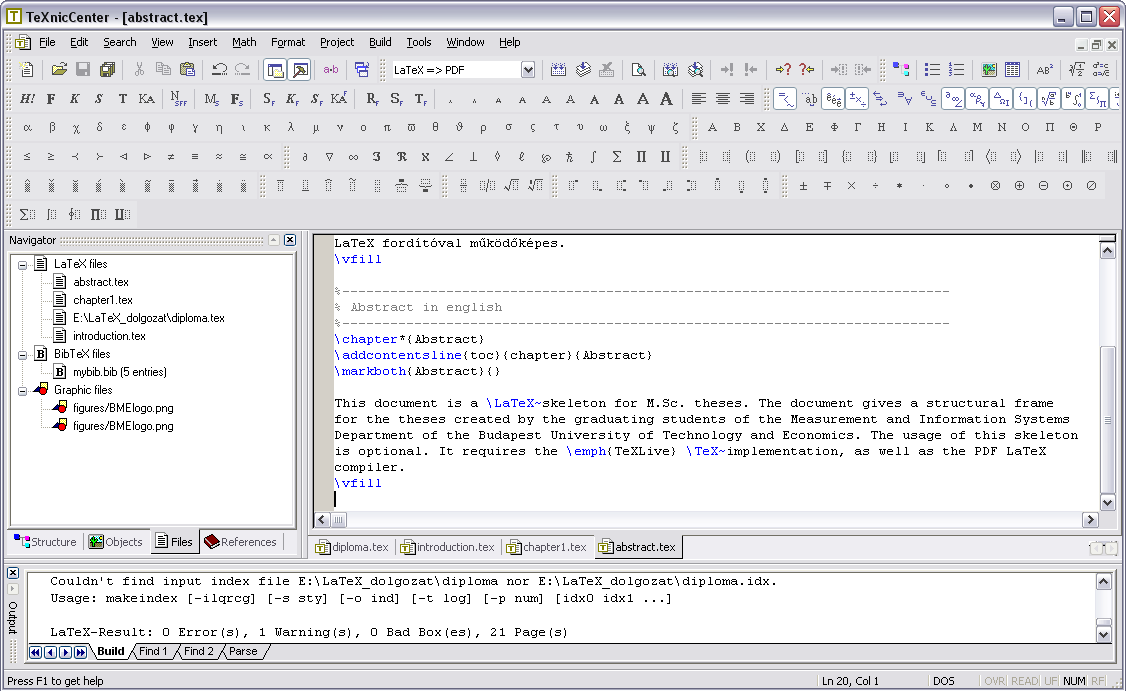
\includegraphics[width=150mm, keepaspectratio]{figures/TeXnicCenter.png}
\caption{A TeXnicCenter Windows alapú \LaTeX-szerkesztõ.} 
\label{fig:TexnicCenter}
\end{figure}

Egy másik használható Windows alapú szerkesztõprogram a LEd (LaTeX Editor,\\\url{http://www.latexeditor.org/}), a TeXnicCenter azonban stabilabb, gyorsabb, és jobban használható.

%----------------------------------------------------------------------------
\section{A dokumentum lefordítása Windows alatt}
%----------------------------------------------------------------------------
A TeXnicCenter és a LEd kizárólag szerkesztõprogram (bár az utóbbiban DVI-nézegetõ is van), így a dokumentum fordításához szükséges eszközöket nem tartalmazza. Windows alatt alapvetõen két lehetõség közül érdemes választani: MiKTeX (\url{http://miktex.org/}) és TeXLive (\url{http://www.tug.org/texlive/}) programcsomag. Az utóbbi mûködik Mac OS X, GNU/Linux alatt és Unix-származékokon is. A MiKTeX egy alapcsomag telepítése után mindig letölti a használt funkciókhoz szükséges, de lokálisan hiányzó \TeX-csomagokat, míg a TeXLive DVD ISO verzóban férhetõ hozzá. Ez a dokumentum TeXLive 2008 programcsomag segítségével fordult, amelynek DVD ISO verziója a megadott oldalról letölthetõ. A sablon lefordításához a disztribúcióban szereplõ \verb+magyar.ldf+ fájlt a \verb+http://www.math.bme.hu/latex/+ változatra kell cserélni, vagy az utóbbi változatot be kell másolni a projekt-könyvtárba (ahogy ezt meg is tettük a sablonban) különben anomáliák tapasztalhatók a dokumentumban (pl. az ábra- és táblázat-aláírások formátuma nem a beállított lesz, vagy bizonyos oldalakon megjelenik alapételmezésben egy fejléc). A TeXLive 2008-at még nem kell külön telepíteni a gépre, elegendõ DVD-rõl (vagy az ISO fájlból közvetlenül, pl. DaemonTools-szal) használni. 

A \TeX-eszközöket tartalmazó programcsomag binárisainak elérési útját minden esetben be kell állítani a szerkesztõprogramban, például TeXnicCenter esetén legegyszerûbben a \verb+Build / Define output profiles...+ menüponttal elõhívott dialógusablakban a \verb+Wizard...+ gombra kattintva tehetjük ezt meg.

A PDF-\LaTeX~használata esetén a generált dokumentum közvetlenül PDF-formátumban áll rendelkezésre. Amennyiben a PDF-fájl egy PDF-nézõben (pl. Adobe Acrobat Reader vagy Foxit PDF Reader) meg van nyitva, akkor a fájlleírót a PDF-nézõ program tipikusan lefoglalja. Ilyen esetben a dokumentum újrafordítása hibaüzenettel kilép. Ha bezárjuk és újra megnyitjuk a PDF dokumentumot, akkor pedig a PDF-nézõk többsége az elsõ oldalon nyitja meg a dokumentumot, nem a legutóbb olvasott oldalon. Ezzel szemben például az egyszerû és ingyenes \textcolor{blue}{Sumatra PDF} nevû program képes arra, hogy a megnyitott dokumentum megváltozását detektálja, és frissítse a nézetet az aktuális oldal megtartásával.

%----------------------------------------------------------------------------
\section{Eszközök Linuxhoz}
%----------------------------------------------------------------------------
Linux operációs rendszer alatt is rengeteg szerkesztõprogram van, pl. a KDE alapú Kile jól használható. Ez ingyenesen letölthetõ, vagy éppenséggel az adott Linux-disztribúció eleve tartalmazza, ahogyan a dokumentum fordításához szükséges csomagokat is. Az Ubuntu Linux disztribúciók alatt például legtöbbször a \verb+texlive-base+ csomag telepítésével használhatók a \LaTeX-eszközök.

%----------------------------------------------------------------------------
\chapter{A házi feladat megoldása}
%----------------------------------------------------------------------------
%----------------------------------------------------------------------------
\section{Első feladat}
%----------------------------------------------------------------------------
A motort a leírásban részletezett módon modelleztük a PDE toolbox segítségével. Mivel esetünkben, időben változás nincs, így a magnetosztatikai módot választottuk. A motor egyszerűsített modellje egy statorból, rotorból, tekercsekből és légrésből áll. Ezek elrendezését a Matlab parancssorjában adtuk meg, majd mivel az elrendezés a függőleges tengelyre antiszimmetrikus, a vízszintesre pedig szimmetrikus, így elegendő az egyik negyedet modellezni. A jobb felső negyed kiválasztás után összevontuk a megfelelő elemekhez tartozó subdomaineket, ezután pedig megadtuk az így kialakult peremeken a megfelelő peremfeltételeket. A stator külsejére, illetve a  modell függőleges tengelyre illeszkedő peremére Dirichlet peremfeltételt, mert a peremen a mágneses skalárpotenciál nulla, a modell vízszintes tengelyére illeszkedő peremére pedig Neumann peremfeltételt, mert a mágneses skalárpotenciál normális irányú gradiense nulla. Ezután beállítottuk az adott anyagjellemzőket és az áramsűrűséget a tekercsben. Inicializáltuk a rácshálót, majd a \textit{Solve} paramétereknél, nemlineáris \textit{solvert} választva elindítottuk a szimulációt. Az alapértelmezett toleranciahatárra kevésbé voltak megfigyelhetők a későbbi feladatokban a kisebb változások, így a nemlináris \textit{solvert}  $ 10^{-11} $-es tolerancia határra állítottuk.
 \begin{figure}[!h]
	\centering
	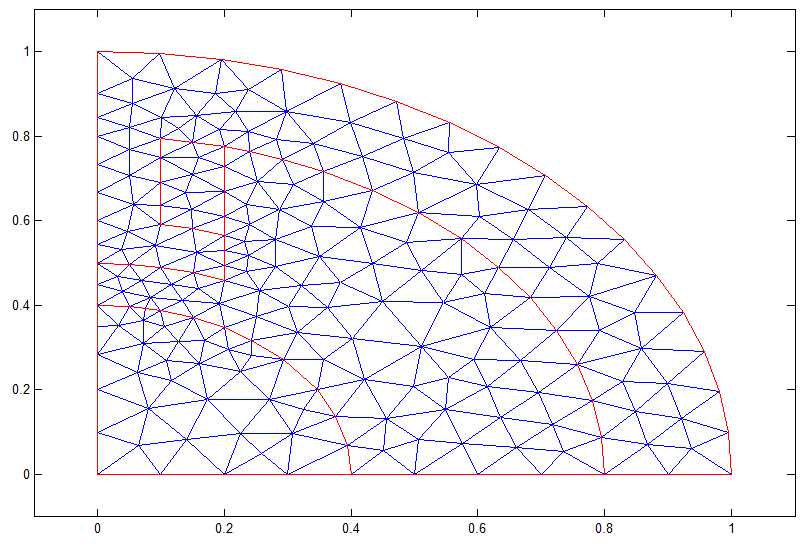
\includegraphics[width=61.5mm, keepaspectratio]{figures/terek/nl_1_init_mesh.png}\hspace{5mm}
	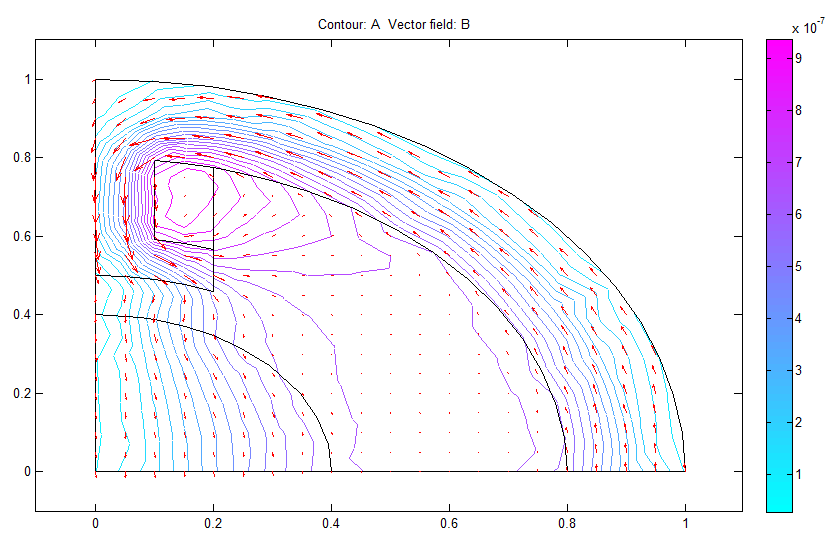
\includegraphics[width=69mm, keepaspectratio]{figures/terek/nl_1_init.png}
	\caption{Az első eredmények}
	\label{fig:calib}
\end{figure}


%----------------------------------------------------------------------------
\section{Második feladat}
%----------------------------------------------------------------------------

A mágneses indukcióvonalak mellett érdemes megvizsgálni, hogy a motoron belül hol mekkora a mágneses indukció abszolútértéke. Ezt mi egy \textit{surface} függvény segítségével ábrázoltuk, mely a \figref{normaleloszlas}~ábrán látható. Miután elvégeztük a modellezést a PDE toolbox segítségével, kiexportáltuk a modellezés során használt háló pontjait, illetve az egyes pontokban a mágneses indukció nagyságát. Az exportált értékeket a \textit{workspace}-ben megjelenítve elkészíthető a 3D-s ábra. Mivel a pontok nem egyenletes távolságra helyezkednek el egymástól, ezért az ábrázoláshoz nem volt lehetséges az ábrázolás egyszerűen csak a \textit{meshgrid} és a \textit{surf} függvények használatával, de a Matlab \textit{griddata} elnevezésű interpoláló függvényével a probléma megoldható. Az abszolút értékek nagyságának leolvasásához egy \textit{colorbar}-t is megjelenítettünk.

\begin{figure}[!h]
	\centering
	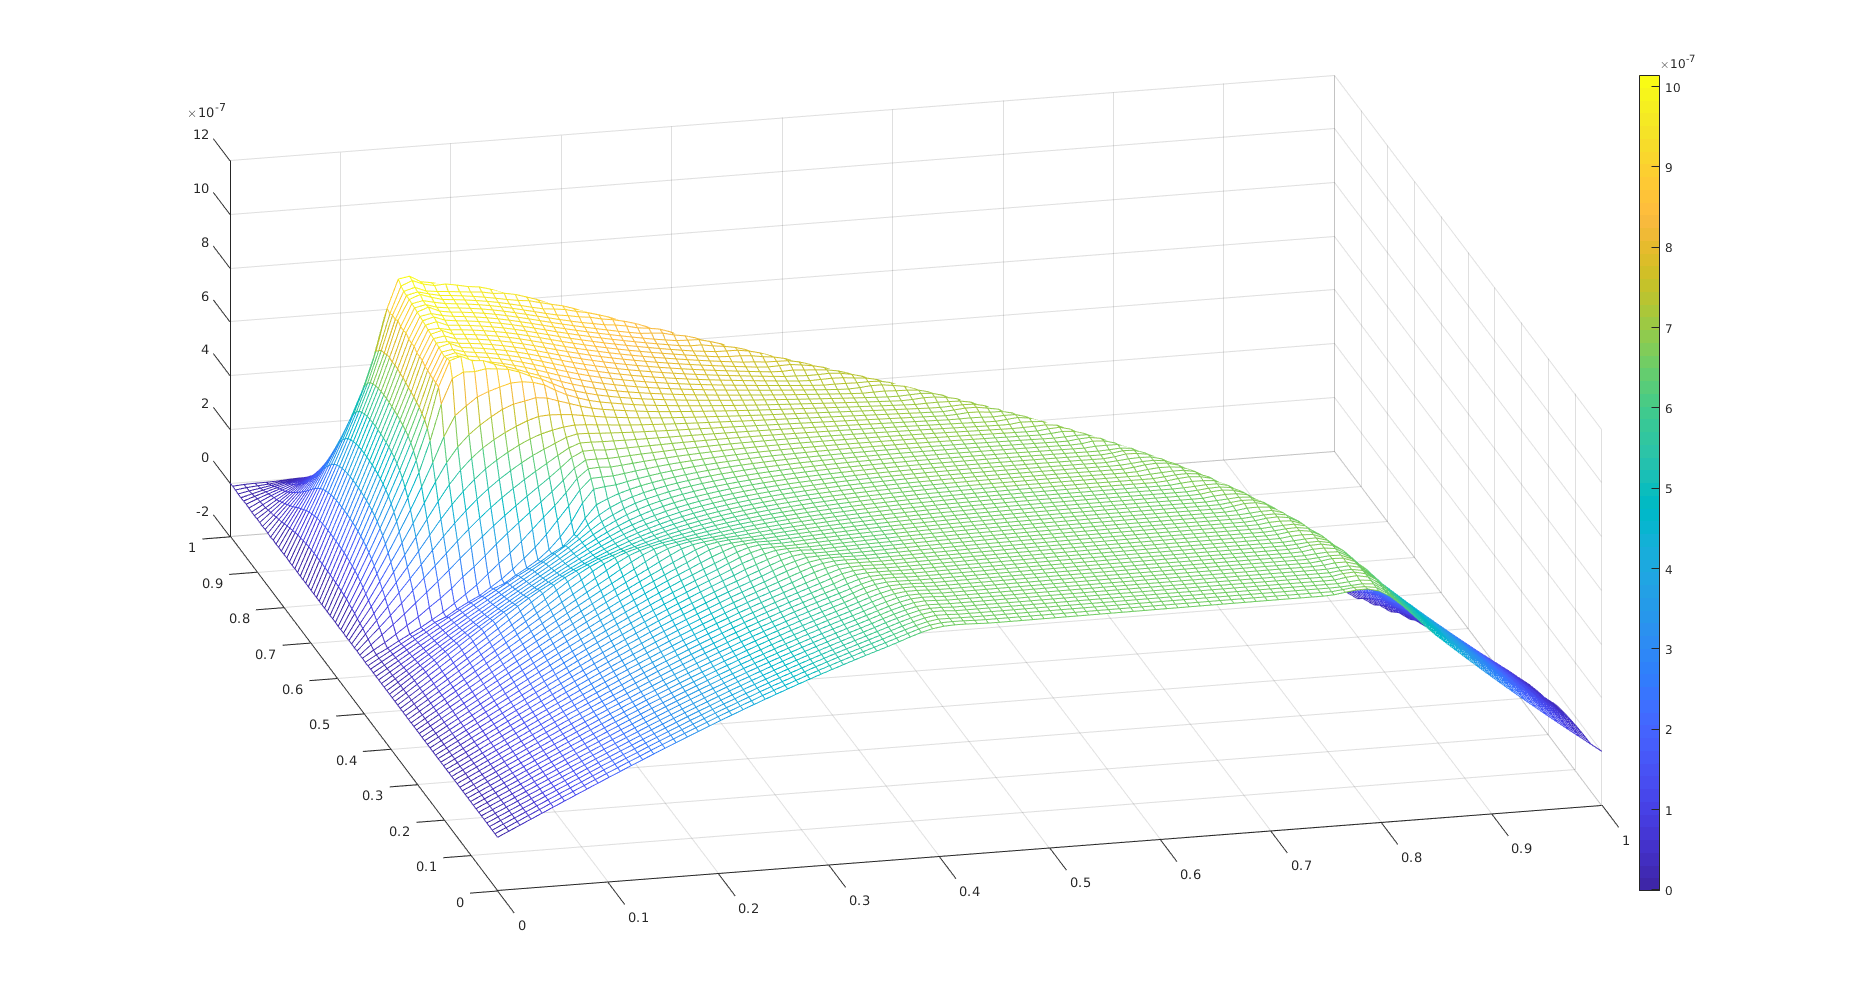
\includegraphics[width=150mm, keepaspectratio]{figures/terek/normal_eloszlas}
	\caption{Mágneses indukció abszolút értékei}
	\label{fig:normaleloszlas}
\end{figure}


Az ábráról leolvasható, hogy a mágneses indukció maximuma  $ 10^{-6} $-on nagyságrendű, és jól látszik, hogy legnagyobb értékek a tekercs közelében tapasztalhatók. Emellett jól megfigyelhető, hogy a stator és a rotor közötti légrésben a tekercstől távolodva a mágneses indukciónak egy „fennsíkja” van, ami kb.  $ 7*10^{-7} $-en értékű. A stator külsején, illetve a függőleges tengely mentén az indukció nagysága 0, ami a peremfeltételekkel összhangban van.
\newpage
%----------------------------------------------------------------------------
\section{Harmadik feladat}
%----------------------------------------------------------------------------
Nemlineáris helyett lineáris vasmagot feltételezve, a modellt így megoldva első ránézésre az indukció abszolút értékeiben nagy változás nem látható, azonban a két felület különbségét képezve az eltérés láthatóvá válik, ezt ábrázoltuk a \figref{kulonbseg}~ábrán.

\begin{figure}[!h]
	\centering
	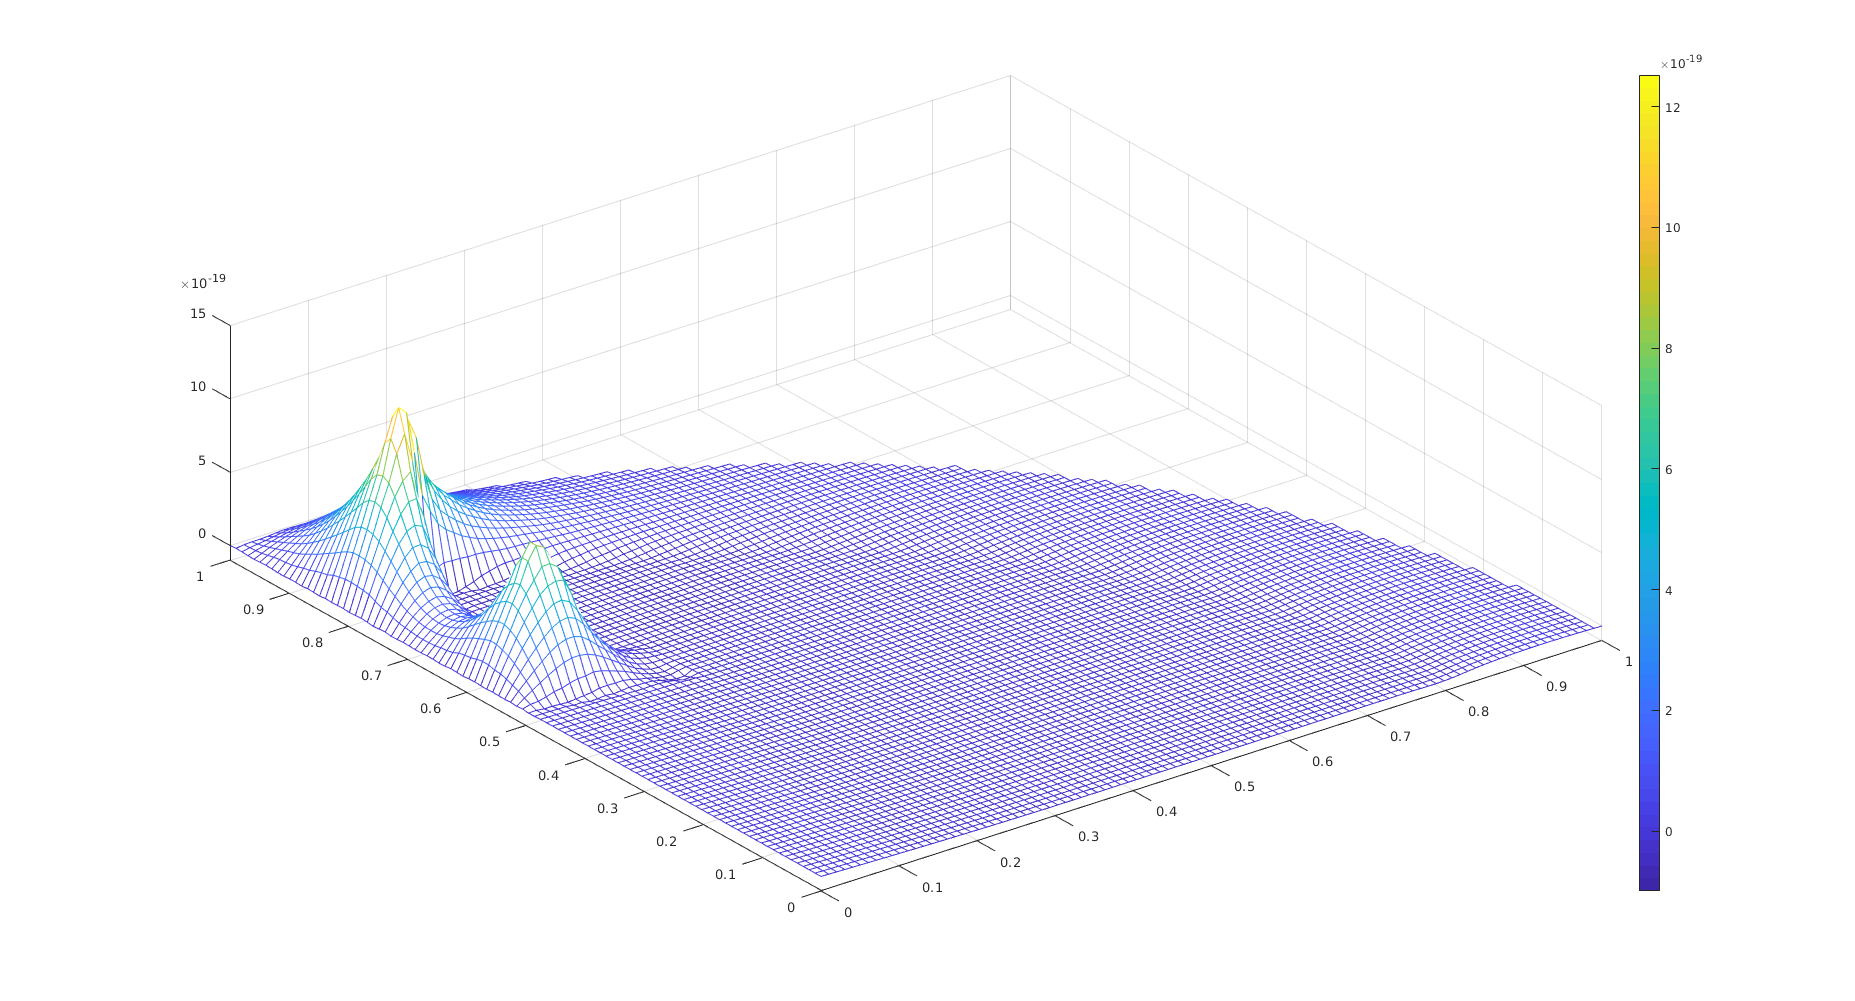
\includegraphics[width=150mm, keepaspectratio]{figures/terek/kulonbseg}
	\caption{A mágneses indukciók nagyságainak különbsége lineáris és nemlineáris vas esetén}
	\label{fig:kulonbseg}
\end{figure}

Megfigyelhető, hogy a legnagyobb eltérés a tekercsnél, azon belül is a tekercs sarkainál tapasztalható. A maximális eltérés a lineáris és a nemlineáris vas között $ 10^{-18} $-on nagyságrendbe esik.




%----------------------------------------------------------------------------
\section{Negyedik feladat}
%----------------------------------------------------------------------------

A PDE ToolBoxban számos lehetőség van a végeselem számítás/(szimuláció?) pontosítására, finomabb végeselemháló készítésére. A háló jóságának egyik jellemzője az őt alkotó háromszögek milyensége. Ez egy 0 és 1 közötti szám, minél nagyobb, annál jobban hasonlít az adott háromszög egy egyenlőoldalú háromszögre. A PDE Toolboxban megtalálható egy \textit{„Jiggle Mesh”} funkció, mely egyenletesebben oszlatja el a csúcspontokat, jobb minőségű háromszögeket alkotva. Ez a funkció a paraméterekben állítható változóval akár többször is lefuttatható, így már a kezdeti háló is javítható a \figref{jiggle} ábrán látható módon.
\begin{figure}[!h]
	\centering
	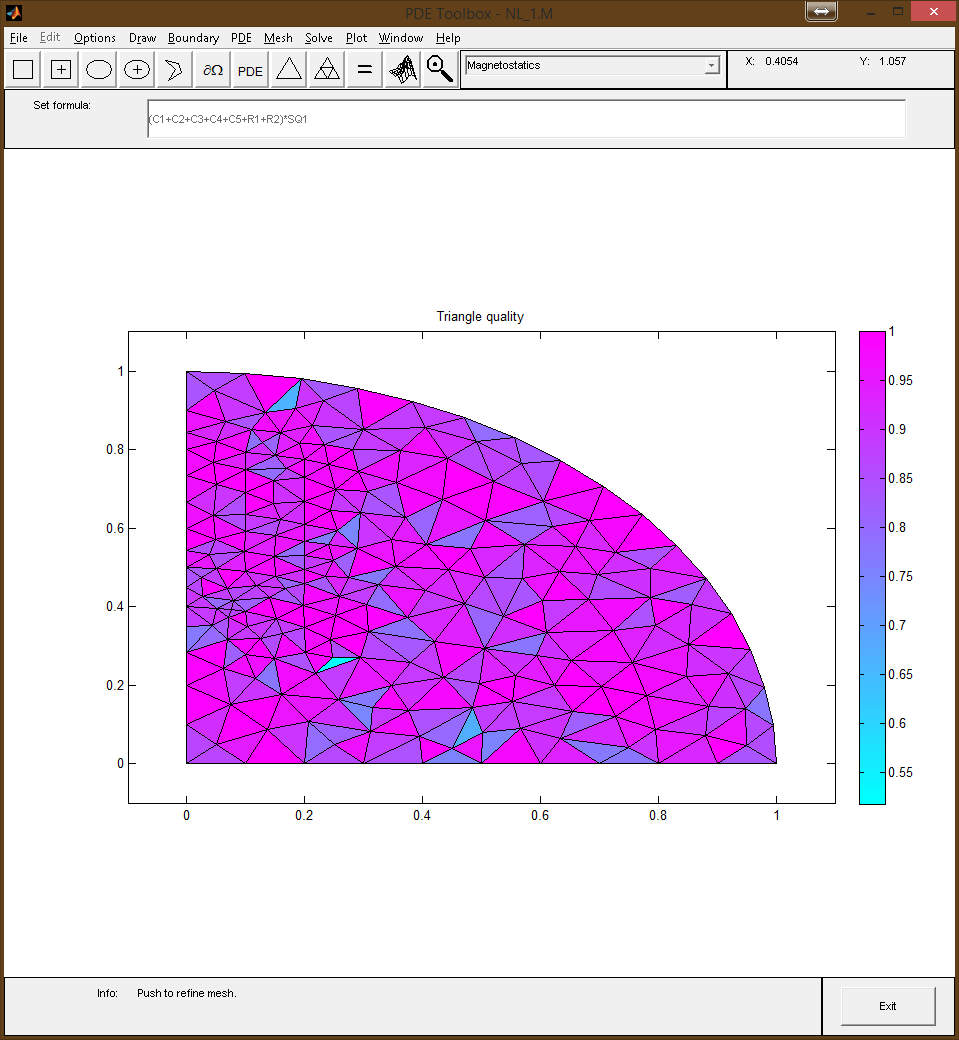
\includegraphics[trim = 25mm 50mm 10mm 70mm,clip, width=69mm, keepaspectratio]{figures/terek/nl_1_3szog0.png}\hspace{5mm}
	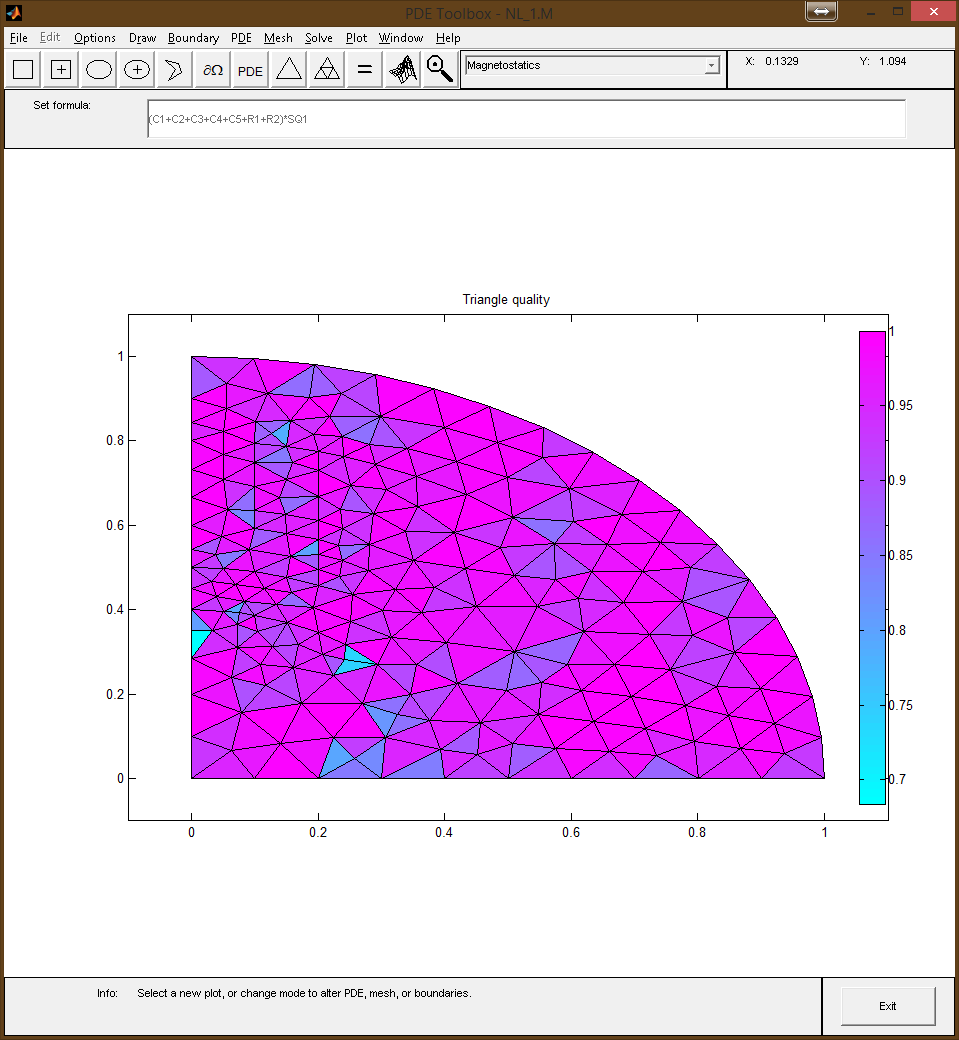
\includegraphics[trim = 25mm 50mm 10mm 70mm,clip, width=67mm, keepaspectratio]{figures/terek/nl_1_3szog1.png}
	\caption{A jiggle nélküli, illetve az azt futtató háló háromszögeinek minőségei}
	\label{fig:jiggle}
\end{figure}

A \textit{„Refine Mesh”} funkcióhoz két paraméter tartozik, az elsővel beállítható, hogy milyen módszerrel finomítsunk a hálón, a másodikkal pedig a növekedési ráta állítható. Az általános esetben a háromszögek oldalainak felezőpontjait összekötve alkot új háromszögeket a toolbox, értelemszerűen így megnégyszerezve az elemek számát, a \textit{longest} módban pedig a háromszög átfogójának felezőpontját a vele szemközti csúccsal köti össze, így megduplázza az elemek számát. Utóbbi módban a növekedési ráta paraméterrel nem csak az eddig meglévő, de már az újonnan létrejött háromszögek egy részén is finomítani lehet egy iteráció alatt.

Ezeken felül lehetőség van az Adaptív végeselemháló finomításhoz, mely a \textit{Solve} paraméterek között kapcsolható be. Itt beállíthatjuk, hogy a szimuláció során mennyi finomítást végezzen a program, azokat milyen módon, illetve mely háromszögekre alkalmazva. A toolbox a legrosszabb minőségű háromszögeket vagy a szomszédos háromszögekhez képest a legnagyobb relatív különbséget elérő(?) háromszögeket finomítja, melyekhez toleranciát is lehet beállítani. Itt több paramétert célszerű kipróbálni, ugyanis túl kis tolerancia esetén az összes háromszögen, túl nagy tolerancia esetén pedig egyiken se fog finomítani az algoritmus. A \figref{adaptive}~ábrán ugyanazon kezdeti hálózat finomítása látható 2 iteráció után, adaptív finomítás nélküli, illetve azt alkalmazó esetben. Látható, hogy a tekercshez közelebb, ahol nagyobbak a mágneses indukció értékei ott a rácshálót is sűrűbben vette fel a program.


\begin{figure}[!h]
	\centering
	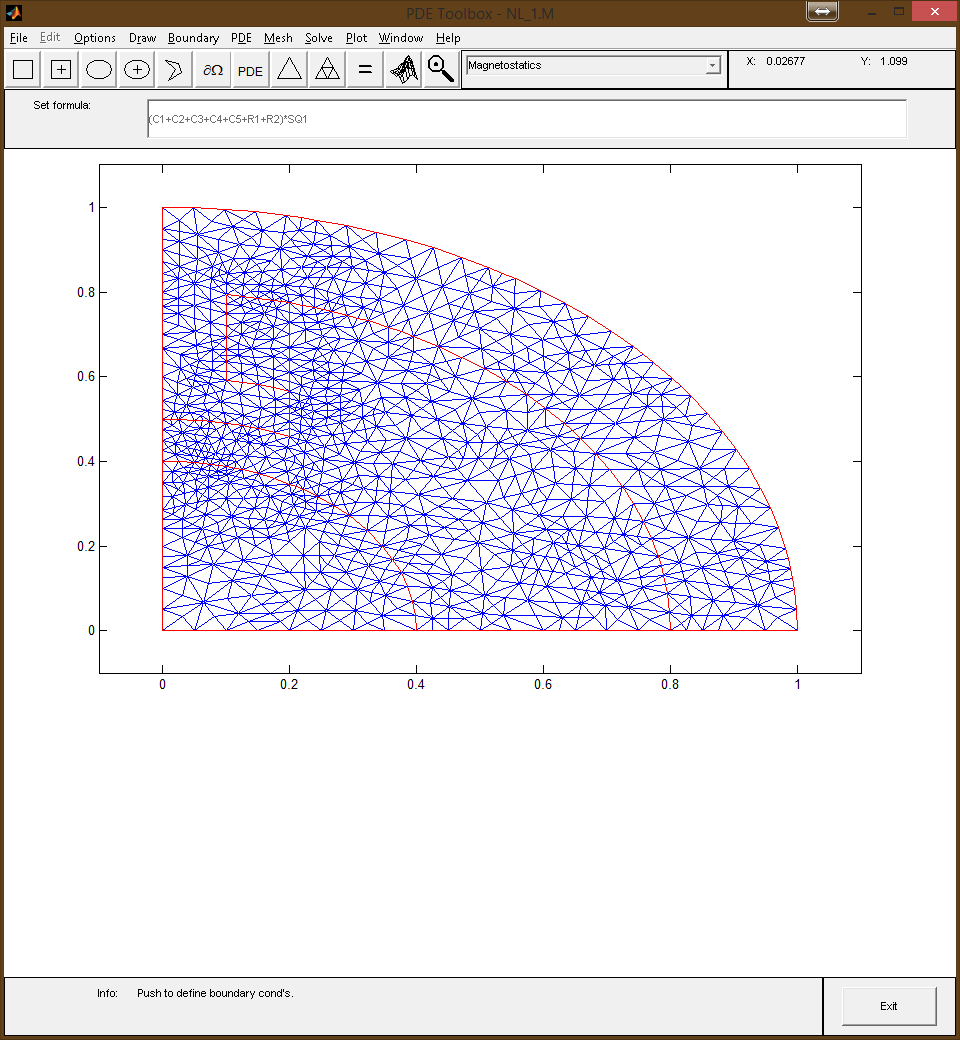
\includegraphics[trim = 15mm 80mm 10mm 40mm,clip, width=69mm, keepaspectratio]{figures/terek/mesh1.png}\hspace{5mm}
	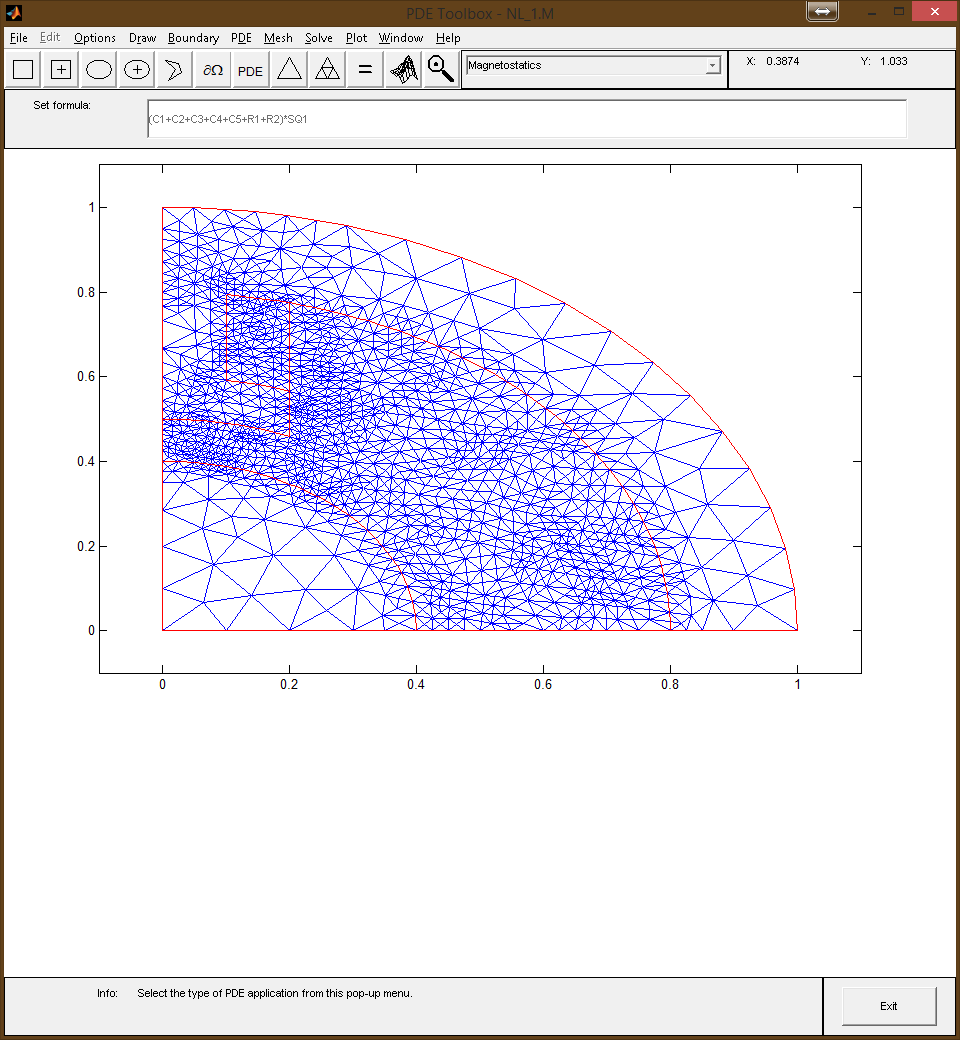
\includegraphics[trim = 15mm 80mm 10mm 40mm,clip, width=69mm, keepaspectratio]{figures/terek/mesh2.png}
	\caption{Adaptív finomítás}
	\label{fig:adaptive}
\end{figure}
\newpage
Ezen ismeretekre alapozva meghatároztunk 4 féle végeselemháló finomítási módot, melyek a következők:


\begin{enumerate}
	\item Nem adaptív, \textit{jiggle} nélküli, \textit{longest} módszerű, 1.3-as növekedési rátával.
	\item Nem adaptív, 20 \textit{jiggle}-t futtató, általános módszerű.
	\item Adaptív, maximum 2000 finomítást, $ 10^{-7} $-es toleranciát használó \textit{longest} módszerű.
	\item Adaptív, maximum 2000 finomítást, $ 10^{-7} $-es toleranciát használó általános módszerű.
\end{enumerate}
Ezeket mind a lineáris, mind a nemlineáris modellre lefuttattuk, az eredményeket kiexportáltuk, és megkerestük a mágneses indukció értékek maximumát. Eredményeink a \tabref{res-lin} és a \tabref{res-nl} táblázatokban találhatóak. Látható, hogy az általános felezőpontos módszer könnyebben megtalálja a felület maximumát, ám az adaptív finomítást használva ez akár lényegesen kevesebb háromszöggel is elérhető.

\begin{table}[!h]
	\centering
	\begin{tabular}{|c||c|c|c|c|}
		\hline
		\textbf{$ *10^{-6} $}		&1. mód&    2. mód&    3. mód&    4. mód\\ \hline\hline
		Inicializáció&   0.96196865034802&   0.96312399284637&   0.98312171335652&   0.98320005165117\\ \hline
		1. Iteráció&   0.97675147818946&   0.98320723184013&   0.98777832396964&   0.99108471276693\\ \hline
		2. Iteráció&   0.98299702428866&   0.99109788082421&   0.99140497343270&   0.99418851293672\\ \hline
		3. Iteráció&   0.98886512022438&   0.99420673120022&   0.99341595180488&   0.99544815538382\\ \hline
		4. Iteráció&   0.99132744744480&   0.99546873795444&   0.99443044519884&   0.99595287564214\\ \hline
		
	\end{tabular}
	\caption{A mágneses indukció maximumértékének változása lineáris modell esetén}
	\label{tab:res-lin}
\end{table}

\begin{table}[!h]
	\centering
\begin{tabular}{|c||c|c|c|c|}
	\hline
	\textbf{$ *10^{-6} $}		&1. mód&    2. mód&    3. mód&    4. mód\\ \hline\hline
	Inicializáció&   0.96196865034802&   0.96312399284635&   0.98312171335651&   0.98320005165113\\ \hline
	1. Iteráció&   0.97675147818948&   0.98320723184012&   0.98777832396964&   0.99108471276696\\ \hline
	2. Iteráció&   0.98299702428871&   0.99109788082414&   0.99140497343272&   0.99418851293635\\ \hline
	3. Iteráció&   0.98886512022444&   0.99420673120021&   0.99341595180488&   0.99544815538414\\ \hline
	4. Iteráció&   0.99132744744506&   0.99546873795697&   0.99443044519850&   0.99595287564182\\ \hline
	
\end{tabular}
\caption{A mágneses indukció maximumértékének változása nemlineáris modell esetén}
\label{tab:res-nl}
\end{table}

\begin{table}[!h]
	\centering
	\begin{tabular}{|c||c|c|c|c|}
		\hline
				&1. mód&    2. mód&    3. mód&    4. mód\\ \hline\hline
		Inicializáció&371&371&1539&1210\\ \hline
		1. Iteráció&902&1484&2932&3888\\ \hline
		2. Iteráció&2059&5936&5628&12943\\ \hline
		3. Iteráció&4546&23744&10972&46215\\ \hline
		4. Iteráció&9813&94976&21345&154082\\ \hline
		
		
	\end{tabular}
	\caption{A végeselem hálót alkotó háromszögek száma}
	\label{tab:res-size}
\end{table}






















%%----------------------------------------------------------------------------
\chapter{A \LaTeX-sablon használata}
%----------------------------------------------------------------------------
Ebben a fejezetben röviden, implicit módon bemutatjuk a sablon használatának módját, ami azt jelenti, hogy sablon használata ennek a dokumentumnak a forráskódját tanulmányozva válik teljesen világossá. Amennyiben a szoftver-keretrendszer telepítve van, a sablon alkalmazása és a dolgozat szerkesztése \LaTeX-ben a sablon segítségével tapasztalataink szerint jóval hatékonyabb, mint egy WYSWYG (\emph{What You See is What You Get}) típusú szövegszerkesztõ esetén (pl. Microsoft Word, OpenOffice).

%----------------------------------------------------------------------------
\section{Címkék és hivatkozások}
%----------------------------------------------------------------------------
A \LaTeX~dokumentumban címkéket (\verb+\label+) rendelhetünk ábrákhoz, táblázatokhoz, fejezetekhez, listákhoz, képletekhez stb. Ezekre a dokumentum bármely részében hivatkozhatunk, a hivatkozások automatikusan feloldásra kerülnek.

A sablonban makrókat definiáltunk a hivatkozások megkönnyítéséhez. Ennek megfelelõen minden ábra (\emph{figure}) címkéje \verb+fig:+ kulcsszóval kezdõdik, míg minden táblázat (\emph{table}), képlet (\emph{equation}), fejezet (\emph{section}) és lista (\emph{listing}) rendre a \verb+tab:+, \verb+eq:+, \verb+sect:+ és \verb+listing:+ kulcsszóval kezdõdik, és a kulcsszavak után tetszõlegesen választott címke használható. Ha ezt a konvenciót betartjuk, akkor az elõbbi objektumok számára rendre a \verb+\figref+, \verb+\tabref+, \verb+\eqref+, \verb+\sectref+ és \verb+\listref+ makrókkal hivatkozhatunk. A makrók paramétere a címke, amelyre hivatkozunk (a kulcsszó nélkül). Az összes említett hivatkozástípus, beleértve az \verb+\url+ kulcsszóval bevezetett web-hivatkozásokat is a  \verb+hyperref+\footnote{Segítségével a dokumentumban megjelenõ hivatkozások nem csak dinamikussá válnak, de színezhetõk is, bõvebbet errõl a csomag dokumentációjában találunk. Ez egyúttal egy példa lábjegyzet írására.} csomagnak köszönhetõen aktívak a legtöbb PDF-nézegetõben, rájuk kattintva a dokumentum megfelelõ oldalára ugrik a PDF-nézõ vagy a megfelelõ linket megnyitja az alapértelmezett böngészõvel. A \verb+hyperref+ csomag a kimeneti PDF-dokumentumba könyvjelzõket is készít a tartalomjegyzékbõl. Ez egy szintén aktív tartalomjegyzék, amelynek elemeire kattintva a nézegetõ behozza a kiválasztott fejezetet.

%----------------------------------------------------------------------------
\section{Ábrák és táblázatok}
%----------------------------------------------------------------------------
A képeket PDFLaTeX esetén a veszteségmentes PNG, valamint a veszteséges JPEG formátumban érdemes elmenteni. Az EPS (PostScript) vektorgrafikus képformátum beillesztését a PDFLatex közvetlenül nem támogatja. Ehelyett egy lehetõség 200 dpi, vagy annál nagyobb felbontásban raszterizálni a képet, és PNG formátumban elmenteni. Az egyes képek mérete általában nem, de sok kép esetén a dokumentum összmérete így már szignifikáns is lehet. A dokumentumban felhasznált képfájlokat a dokumentum forrása mellett érdemes tartani, archiválni, mivel ezek hiányában a dokumentum nem fordul újra. Ha lehet, a vektorgrafikus képeket vektorgrafikus formátumban is érdemes elmenteni az újrafelhasználhatóság (az átszerkeszthetõség) érdekében.

Kapcsolási rajzok legtöbbször kimásolhatók egy vektorgrafikus programba (pl. CorelDraw) és onnan nagyobb felbontással raszterizálva kimenthatõk PNG formátumban. Ugyanakkor kiváló ábrák készíthetõk Microsoft Visio vagy hasonló program használatával is: Visio-ból az ábrák közvetlenül PNG-be is menthetõk.

Lehetõségeink Matlab ábrák esetén:
\begin{itemize}
	\item Képernyõlopás (\emph{screenshot}) is elfogadható minõségû lehet a dokumentumban, de általában jobb felbontást is el lehet érni más módszerrel.
	\item A Matlab ábrát a \verb+File/Save As+ opcióval lementhetjük PNG formátumban (ugyanaz itt is érvényes, mint korábban, ezért nem javasoljuk).
	\item A Matlab ábrát az \verb+Edit/Copy figure+ opcióval kimásolhatjuk egy vektorgrafikus programba is és onnan nagyobb felbontással raszterizálva kimenthatjük PNG formátumban (nem javasolt).
	\item Javasolt megoldás: az ábrát a \verb+File/Save As+ opcióval EPS \emph{vektorgrafikus} formátumban elmentjük, PDF-be konvertálva beillesztjük a dolgozatba.
\end{itemize}
Az EPS kép az \verb+epstopdf+ programmal\footnote{a korábban említett \LaTeX-disztribúciókban megtalálható} konvertálható PDF formátumba. Célszerû egy batch-fájlt készíteni az összes EPS ábra lefordítására az alábbi módon (ez Windows alatt mûködik).
\begin{lstlisting}[frame=single,float=!ht]
@echo off
for %%j in (*.eps) do (
echo converting file "%%j"
epstopdf "%%j"
)
echo done .
\end{lstlisting}

Egy ilyen parancsfájlt (\verb+convert.cmd+) elhelyeztük a sablon \verb+figures\eps+ könyvtárába, így a felhasználónak csak annyi a dolga, hogy a \verb+figures\eps+ könyvtárba kimenti az EPS formátumú vektorgrafikus képet, majd lefuttatja a \verb+convert.cmd+ parancsfájlt, ami PDF-be konvertálja az EPS fájlt.

Ezek után a PDF-ábrát ugyanúgy lehet a dokumentumba beilleszteni, mint a PNG-t vagy a JPEG-et. A megoldás elõnye, hogy a lefordított dokumentumban is vektorgrafikusan tárolódik az ábra, így a mérete jóval kisebb, mintha raszterizáltuk volna beillesztés elõtt. Ez a módszer minden -- az EPS formátumot ismerõ -- vektorgrafikus program (pl. CorelDraw) esetén is használható.

A képek beillesztésére az \sectref{LatexTools}. fejezetben mutattunk be példát (\figref{TexnicCenter}~ábra). Az elõzõ mondatban egyúttal az automatikusan feloldódó ábrahivatkozásra is láthatunk példát. Több képfájlt is beilleszthetünk egyetlen ábrába. Az egyes képek közötti horizontális és vertikális margót metrikusan szabályozhatjuk (\figref{HVSpaces}~ábra). Az ábrák elhelyezését számtalan tipográfiai szabály egyidejû teljesítésével a fordító maga végzi, a dokumentum írója csak preferenciáit jelezheti a fordító felé (olykor ez bosszúságot is okozhat, ilyenkor pl. a kép méretével lehet játszani).

\begin{figure}[!ht]
\centering
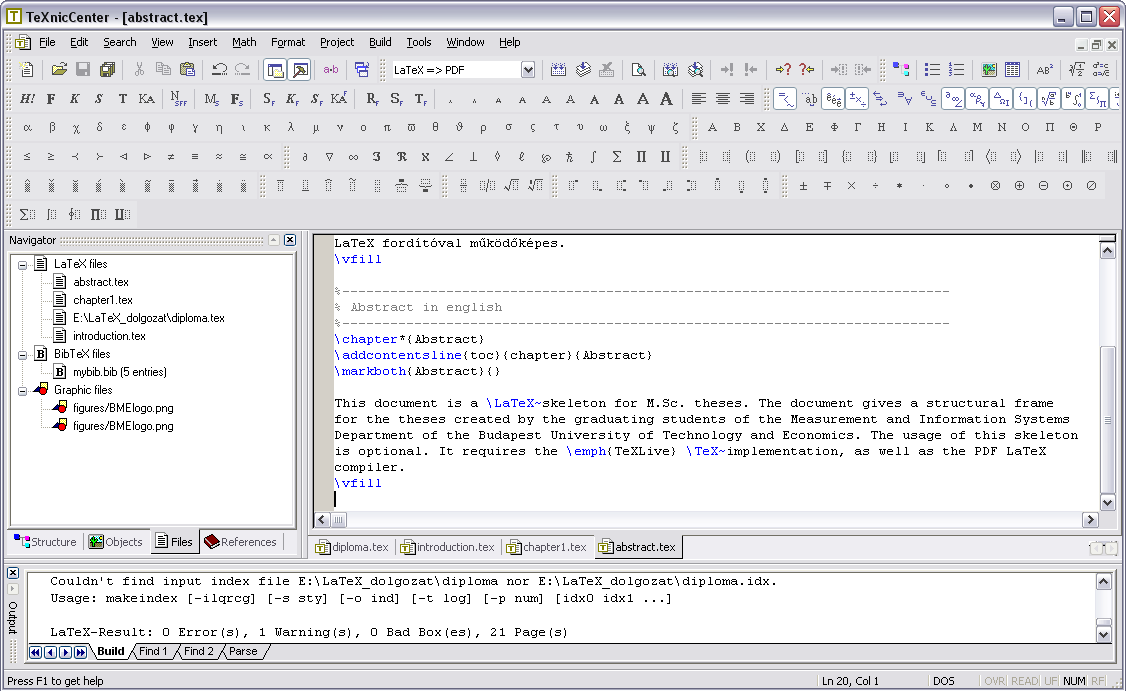
\includegraphics[width=67mm, keepaspectratio]{figures/TeXnicCenter.png}\hspace{1cm}
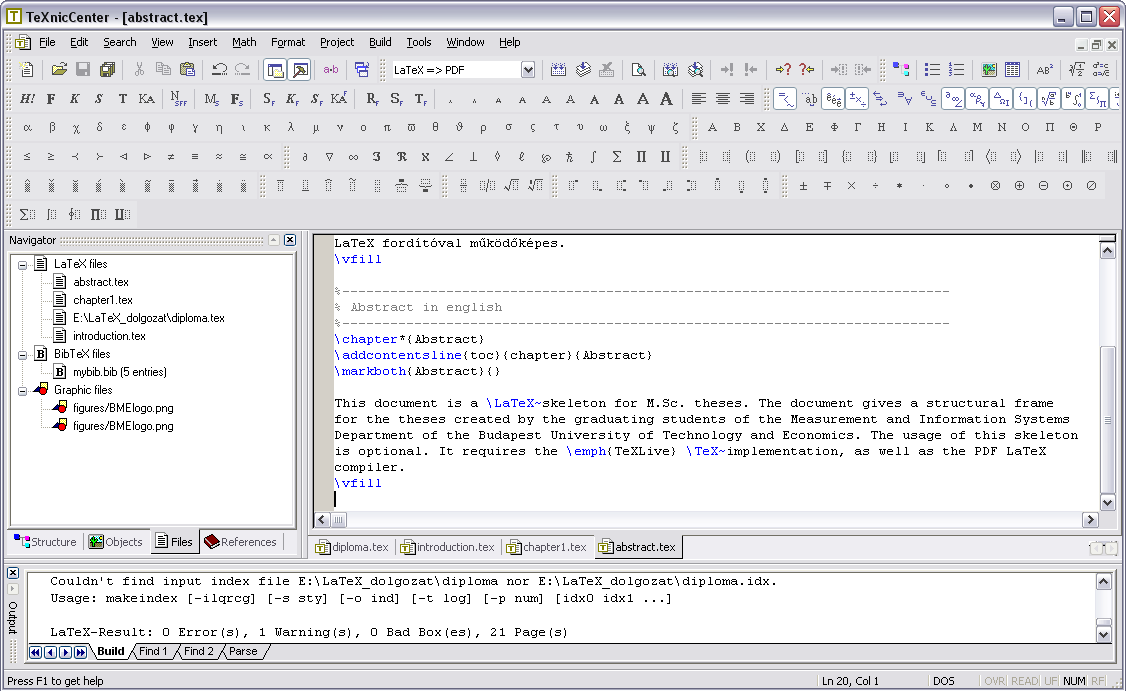
\includegraphics[width=67mm, keepaspectratio]{figures/TeXnicCenter.png}\\\vspace{5mm}
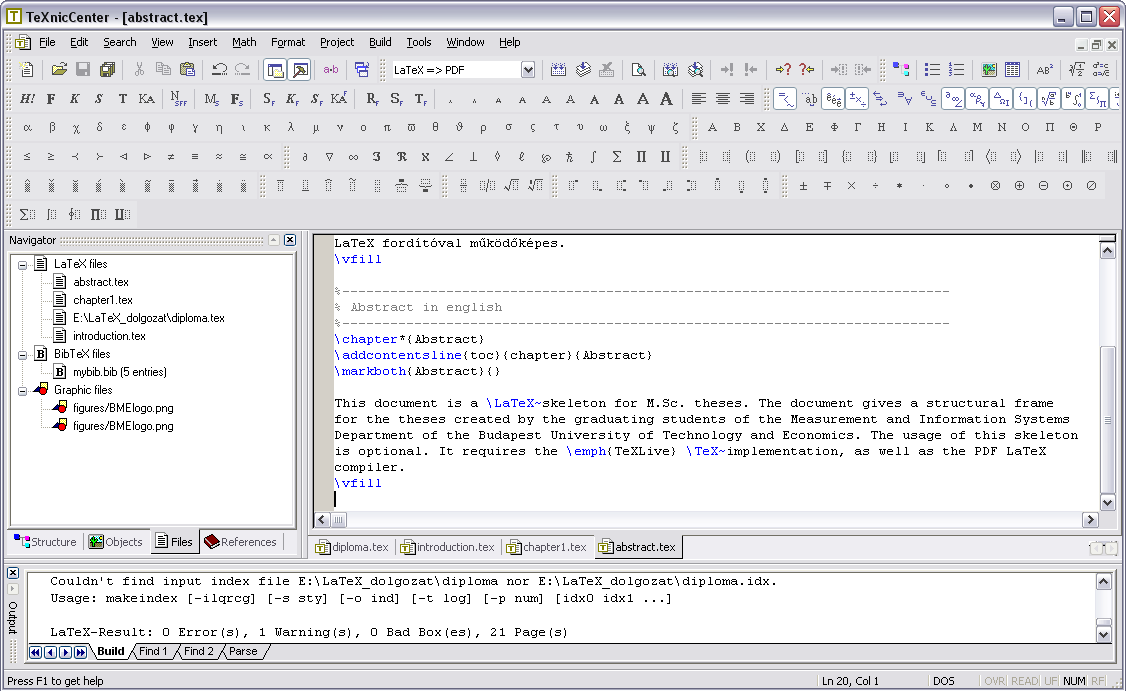
\includegraphics[width=67mm, keepaspectratio]{figures/TeXnicCenter.png}\hspace{1cm}
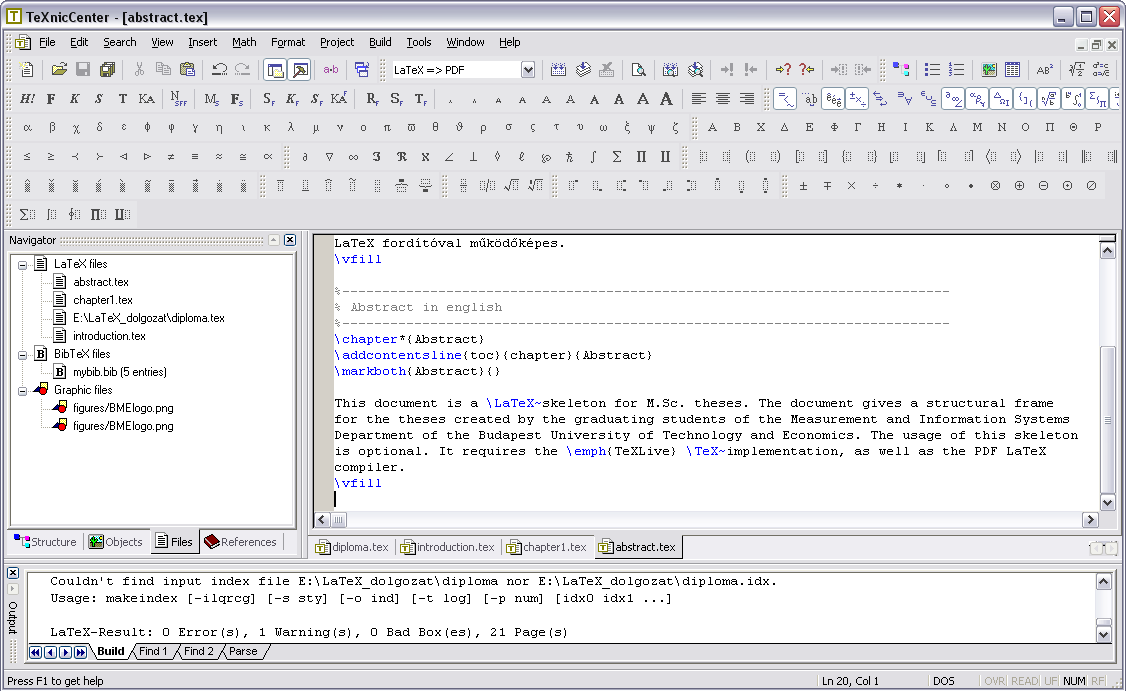
\includegraphics[width=67mm, keepaspectratio]{figures/TeXnicCenter.png}
\caption{Több képfájl beillesztése esetén térközöket is érdemes használni.} 
\label{fig:HVSpaces}
\end{figure}

A táblázatok használatára a \tabref{TabularExample}~táblázat mutat példát.
A táblázat címkéje nem véletlenül került a táblázat fölé, ez a szokványos.
\begin{table}[ht]
	\footnotesize
	\centering
	\caption{Az órajel-generátor chip órajel-kimenetei.} \label{tab:SysClocks}
	\begin{tabular}{ | l | c | c |}
	\hline
	Órajel & Frekvencia & Cél pin \\ \hline
	CLKA & 100 MHz & FPGA CLK0\\
	CLKB & 48 MHz  & FPGA CLK1\\
	CLKC & 20 MHz  & Processzor\\
	CLKD & 25 MHz  & Ethernet chip \\
	CLKE & 72 MHz  & FPGA CLK2\\
	XBUF & 20 MHz  & FPGA CLK3\\
	\hline
	\end{tabular}
	\label{tab:TabularExample}
\end{table}


%----------------------------------------------------------------------------
\section{Felsorolások és listák}
%----------------------------------------------------------------------------
Számozatlan felsorolásra mutat példát a jelenlegi bekezdés:
\begin{itemize}
	\item \emph{elsõ bajusz:} ide lehetne írni az elsõ elem kifejését,
	\item \emph{második bajusz:} ide lehetne írni a második elem kifejését,
	\item \emph{ez meg egy szakáll:} ide lehetne írni a harmadik elem kifejését.
\end{itemize}

Számozott felsorolást is készíthetünk az alábbi módon:
\begin{enumerate}
	\item \emph{elsõ bajusz:} ide lehetne írni az elsõ elem kifejését, és ez a kifejtés így néz ki, ha több sorosra sikeredik,
	\item \emph{második bajusz:} ide lehetne írni a második elem kifejését,
	\item \emph{ez meg egy szakáll:} ide lehetne írni a harmadik elem kifejését.
\end{enumerate}
A felsorolásokban sorok végén vesszõ, az utolsó sor végén pedig pont a szokásos írásjel. Ez alól kivételt képezhet, ha az egyes elemek több teljes mondatot tartalmaznak.

Listákban a dolgozat szövegétõl elkülönítendõ kódrészleteket, programsorokat, pszeudo-kódokat jeleníthetünk meg (\listref{Example}~lista). 
\begin{lstlisting}[frame=single,float=!ht,caption=A fenti számozott felsorolás \LaTeX- forráskódja, label=listing:Example]

\end{lstlisting}
A lista keretét, háttérszínét, egész stílusát megválaszthatjuk. Ráadásul különféle programnyelveket és a nyelveken belül kulcsszavakat is definiálhatunk, ha szükséges. Errõl bõvebbet a \verb+listings+ csomag hivatalos leírásában találhatunk.

%----------------------------------------------------------------------------
\section{Képletek}
%----------------------------------------------------------------------------
Ha egy formula nem túlságosan hosszú, és nem akarjuk hivatkozni a szövegbõl, mint például a $e^{i\pi}+1=0$ képlet, \emph{szövegközi képletként} szokás leírni. Csak, hogy másik példát is lássunk, az $U_i=-d\Phi/dt$ Faraday-törvény a $\rot E=-\frac{dB}{dt}$ differenciális alakban adott Maxwell-egyenlet felületre vett integráljából vezethetõ le. Látható, hogy a \LaTeX-fordító a sorközöket betartja, így a szöveg szedése esztétikus marad szövegközi képletek használata esetén is.

Képletek esetén az általános konvenció, hogy a kisbetûk skalárt, a kis félkövér betûk ($\mathbf{v}$) oszlopvektort -- és ennek megfelelõen $\mathbf{v}^T$ sorvektort -- a kapitális félkövér betûk ($\mathbf{V}$) mátrixot jelölnek. Ha ettõl el szeretnénk térni, akkor az alkalmazni kívánt jelölésmódot célszerû külön alfejezetben definiálni. Ennek megfelelõen, amennyiben $\mathbf{y}$ jelöli a mérések vektorát, $\mathbf{\vartheta}$ a paraméterek vektorát és $\hat{\mathbf{y}}=\mathbf{X}\vartheta$ a paraméterekben lineáris modellt, akkor a \emph{Least-Squares} értelemben optimális paraméterbecslõ $\hat{\mathbf{\vartheta}}_{LS}=(\mathbf{X}^T\mathbf{X})^{-1}\mathbf{X}^T\mathbf{y}$ lesz.

Emellett kiemelt, sorszámozott képleteket is megadhatunk, ennél az \verb+equation+ és a \verb+eqnarray+ környezetek helyett a korszerûbb \verb+align+ környezet alkalmazását javasoljuk (több okból, különféle problémák elkerülése végett, amelyekre most nem térünk ki). Tehát
\begin{align}
\dot{\mathbf{x}}&=\mathbf{A}\mathbf{x}+\mathbf{B}\mathbf{u},\\
\mathbf{y}&=\mathbf{C}\mathbf{x},
\end{align}
ahol $\mathbf{x}$ az állapotvektor, $\mathbf{y}$ a mérések vektora és $\mathbf{A}$, $\mathbf{B}$ és $\mathbf{C}$ a rendszert leíró paramétermátrixok. Figyeljük meg, hogy a két egyenletben az egyenlõségjelek egymáshoz igazítva jelennek meg, mivel a mindkettõt az \& karakter elõzi meg a kódban. Lehetõség van számozatlan kiemelt képlet használatára is, például
\begin{align}
\dot{\mathbf{x}}&=\mathbf{A}\mathbf{x}+\mathbf{B}\mathbf{u},\nonumber\\
\mathbf{y}&=\mathbf{C}\mathbf{x}\nonumber.
\end{align}
Mátrixok felírására az $\mathbf{A}\mathbf{x}=\mathbf{b}$ inhomogén lineáris egyenlet részletes kifejtésével mutatunk példát:
\begin{align}
\begin{bmatrix}
a_{11} & a_{12} & \dots & a_{1n}\\
a_{21} & a_{22} & \dots & a_{2n}\\
\vdots & \vdots & \ddots & \vdots\\
a_{m1} & a_{m2} & \dots & a_{mn}
\end{bmatrix}
\begin{pmatrix}x_1\\x_2\\\vdots\\x_n\end{pmatrix}=
\begin{pmatrix}b_1\\b_2\\\vdots\\b_m\end{pmatrix}.
\end{align}
A \verb+\frac+ utasítás hatékonyságát egy általános másodfokú tag átviteli függvényén keresztül mutatjuk be, azaz
\begin{align}
W(s)=\frac{A}{1+2T\xi s+s^2T^2}.
\end{align}
A matematikai mód minden szimbólumának és képességének a bemutatására természetesen itt nincs lehetõség, de gyors referenciaként hatékonyan használhatók a következõ linkek:\\
\indent\url{http://www.artofproblemsolving.com/LaTeX/AoPS_L_GuideSym.php},\\
\indent\url{http://www.ctan.org/tex-archive/info/symbols/comprehensive/symbols-a4.pdf},\\
\indent\url{ftp://ftp.ams.org/pub/tex/doc/amsmath/short-math-guide.pdf}.\\
Ez pedig itt egy magyarázat, hogy miért érdemes \verb+align+ környezetet használni:\\
\indent\url{http://texblog.net/latex-archive/maths/eqnarray-align-environment/}.

%----------------------------------------------------------------------------
\section{Irodalmi hivatkozások}\label{sect:HowtoReference}
%----------------------------------------------------------------------------
Egy \LaTeX dokumentumban az irodalmi hivatkozások definíciójának két módja van. Az egyik a \verb+\thebibliograhy+ környezet használata a dokumentum végén, az \verb+\end{document}+ lezárás elõtt.
\begin{lstlisting}[frame=single,float=!ht]
\begin{thebibliography}{9}

\bibitem{Lamport94} Leslie Lamport, \emph{\LaTeX: A Document Preparation System}. 
Addison Wesley, Massachusetts, 2nd Edition, 1994.

\end{thebibliography}
\end{lstlisting}

Ezek után a dokumentumban a \verb+\cite{Lamport94}+ utasítással hivatkozhatunk a forrásra. A fenti megadás viszonylag kötetlen, a szerzõ maga formázza az irodalomjegyzéket. 

Egy sokkal professzionálisabb módszer a BiB\TeX~használata, ezért ez a sablon is ezt támogatja. Ebben az esetben egy külön szöveges adatbázisban definiáljuk a forrásmunkákat, és egy külön stílusfájl határozza meg az irodalomjegyzék kinézetét. Ez, összhangban azzal, hogy külön formátumkonvenció határozza meg a folyóirat-, a könyv-, a konferenciacikk- stb. hivatkozások kinézetét az irodalomjegyzékben (a sablon használata esetén ezzel nem is kell foglalkoznia a hallgatónak, de az eredményt célszerû ellenõrizni). A felhasznált hivatkozások adatbázisa egy \verb+.bib+ kiterjesztésû szöveges fájl, amelynek szerkezetét a \listref{Bibtex} kódrészlet demonstrálja. A forrásmunkák bevitelekor a sor végi vesszõk külön figyelmet igényelnek, mert hiányuk a BiB\TeX-fordító hibaüzenetét eredményezi. A forrásmunkákat típus szerinti kulcsszó vezeti be (\verb+@book+ könyv, \verb+@inproceedings+ konferenciakiadványban megjelent cikk, \verb+@article+ folyóiratban megjelent cikk, \verb+@techreport+ valamelyik egyetem gondozásában megjelent mûszaki tanulmány, \verb+@manual+ mûszaki dokumentáció esetén stb.). Nemcsak a megjelenés stílusa, de a kötelezõen megadandó mezõk is típusról-típusra változnak. Egy jól használható referencia a \url{http://en.wikipedia.org/wiki/BibTeX} oldalon található.
\begin{lstlisting}[frame=single,float=!ht,caption=Példa szöveges irodalomjegyzék-adatbázisra BiBTeX használata esetén., label=listing:Bibtex]

\end{lstlisting}

A stílusfájl egy \verb+.sty+ kiterjesztésû fájl, de ezzel lényegében nem kell foglalkozni, mert vannak beépített stílusok, amelyek jól használhatók. Ez a sablon a BiB\TeX-et használja, a hozzá tartozó adatbázisfájl a \verb+mybib.bib+ fájl. Megfigyelhetõ, hogy az irodalomjegyzéket a dokumentum végére (a \verb+\end{document}+ utasítás elé) beillesztett \verb+\bibliography{mybib}+ utasítással hozhatjuk létre, a stílusát pedig ugyanitt a  \verb+\bibliographystyle{plain}+ utasítással adhatjuk meg. Ebben az esetben a \verb+plain+ elõre definiált stílust használjuk (a sablonban is ezt állítottuk be). A \verb+plain+ stíluson kívül természetesen számtalan más elõre definiált stílus is létezik. Mivel a \verb+.bib+ adatbázisban ezeket megadtuk, a BiB\TeX-fordító is meg tudja különböztetni a szerzõt a címtõl és a kiadótól, és ez alapján automatikusan generálódik az irodalomjegyzék a stílusfájl által meghatározott stílusban.

Az egyes forrásmunkákra a szövegbõl továbbra is a \verb+\cite+ paranccsal tudunk hivatkozni, így a \listref{Bibtex} kódrészlet esetén a hivatkozások rendre \verb+\cite{Wettl04}+, \verb+\cite{Candy86}+, \verb+\cite{Lee87}+, \verb+\cite{KissPhD}+, \verb+\cite{Schreirer00}+ és \verb+\cite{DipPortal}+. Az irodalomjegyzékben alapértelmezésben csak azok a forrásmunkák jelennek meg, amelyekre található hivatkozás a szövegben, és ez így alapvetõen helyes is, hiszen olyan forrásmunkákat nem illik az irodalomjegyzékbe írni, amelyekre nincs hivatkozás.

Mivel a fordítási folyamat során több lépésben oldódnak fel a szimbólumok, ezért gyakran többször (TeXLive és TeXnicCenter esetén 2-3-szor) is le kell fordítani a dokumentumot. Ilyenkor ez elsõ 1-2 fordítás esetleg szimbólum-feloldásra vonatkozó figyelmeztetõ üzenettel zárul. Ha hibaüzenettel zárul bármelyik fordítás, akkor nincs értelme megismételni, hanem a hibát kell megkeresni. A \verb+.bib+ fájl megváltoztatáskor sokszor nincs hatása a változtatásnak azonnal, mivel nem mindig fut újra a BibTeX fordító. Ezért célszerû a változtatás után azt manuálisan is lefuttatni (TeXnicCenter esetén \verb+Build/BibTeX+).

Hogy a szövegbe ágyazott hivatkozások kinézetét demonstráljuk, itt most sorban meghivatkozzuk a \cite{Wettl04}, \cite{Candy86}, \cite{Lee87}, \cite{KissPhD} és az \cite{Schreier00} forrásmunkát, valamint az \cite{DipPortal} weboldalt.

Megjegyzendõ, hogy az ékezetes magyar betûket is tartalmazó \verb+.bib+ fájl az \verb+inputenc+ csomaggal betöltött \verb+latin2+ betûkészlet miatt fordítható. Ugyanez a \verb+.bib+ fájl hibaüzenettel fordul egy olyan dokumentumban, ami nem tartalmazza a \verb+\usepackage[latin2]{inputenc}+ sort. Speciális igény esetén az irodalmi adatbázis általánosabb érvényûvé tehetõ, ha az ékezetes betûket speciális latex karakterekkel helyettesítjük a \verb+.bib+ fájlban, pl. á helyett \verb+\'{a}+-t vagy õ helyett \verb+\H{o}+-t írunk. 

Oldaltörés következik (ld. forrás).
\newpage

%----------------------------------------------------------------------------
\section{A dolgozat szerkezete és a forrásfájlok}
%----------------------------------------------------------------------------
A diplomatervsablon (a kari irányelvek szerint) az alábbi fõ fejezetekbõl áll:
\begin{enumerate}
	\item 1 oldalas \emph{tájékoztató} a szakdolgozat/diplomaterv szerkezetérõl (\verb+guideline.tex+), ami a végsõ dolgozatból törlendõ,
	\item \emph{feladatkiírás} (\verb+project.tex+), a dolgozat nyomtatott verzójában ennek a helyére kerül a tanszék által kiadott, a tanszékvezetõ által aláírt feladatkiírás, a dolgozat elektronikus verziójába pedig a feladatkiírás egyáltalán ne kerüljön bele, azt külön tölti fel a tanszék a diplomaterv-honlapra,
	\item \emph{címoldal} (\verb+titlepage.tex+),
	\item \emph{tartalomjegyzék} (\verb+diploma.tex+),
	\item a diplomatervezõ \emph{nyilatkozat}a az önálló munkáról (\verb+declaration.tex+),
	\item 1-2 oldalas tartalmi \emph{összefoglaló} magyarul és angolul, illetve elkészíthetõ még további nyelveken is (\verb+abstract.tex+),
	\item \emph{bevezetés}: a feladat értelmezése, a tervezés célja, a feladat indokoltsága, a diplomaterv felépítésének rövid összefoglalása (\verb+introduction.tex+),
	\item sorszámmal ellátott \emph{fejezetek}: a feladatkiírás pontosítása és részletes elemzése, elõzmények (irodalomkutatás, hasonló alkotások), az ezekbõl levonható következtetések, a tervezés részletes leírása, a döntési lehetõségek értékelése és a választott megoldások indoklása, a megtervezett mûszaki alkotás értékelése, kritikai elemzése, továbbfejlesztési lehetõségek (\verb+chapter{1,2..n}.tex+),
	\item esetleges \emph{köszönetnyilvánítás}ok (\verb+acknowledgement.tex+),
	\item részletes és pontos \emph{irodalomjegyzék} (ez a sablon esetében automatikusan generálódik a \verb+diploma.tex+ fájlban elhelyezett \verb+\bibliography+ utasítás hatására, a \sectref{HowtoReference}. fejezetben leírtak szerint),
	\item \emph{függelékek} (\verb+appendices.tex+).
\end{enumerate}

A sablonban a fejezetek a \verb+diploma.tex+ fájlba vannak beillesztve \verb+\include+ utasítások segítségével. Lehetõség van arra, hogy csak az éppen szerkesztés alatt álló \verb+.tex+ fájlt fordítsuk le, ezzel lerövidítve a fordítási folyamatot. Ezt a lehetõséget az alábbi kódrészlet biztosítja a \verb+diploma.tex+ fájlban.
\begin{lstlisting}[frame=single,float=!ht]
\includeonly{
	guideline,%
	project,%
	titlepage,%
	declaration,%
	abstract,%
	introduction,%
	chapter1,%
	chapter2,%
	chapter3,%
	acknowledgement,%
	appendices,%
}
\end{lstlisting}

Ha az alábbi kódrészletben az egyes sorokat a \verb+%+ szimbólummal kikommentezzük, akkor a megfelelõ \verb+.tex+ fájl nem fordul le. Az oldalszámok és a tartalomjegyék természetesen csak akkor billennek helyre, ha a teljes dokumentumot lefordítjuk.

%----------------------------------------------------------------------------
\newpage
\section{Alapadatok megadása}
%----------------------------------------------------------------------------
A diplomaterv alapadatait (cím, szerzõ, konzulens, konzulens titulusa) a \verb+diploma.tex+ fájlban lehet megadni az alábbi kódrészlet módosításával.


%----------------------------------------------------------------------------
\section{Új fejezet írása}
%----------------------------------------------------------------------------
A fõfejezetek külön \verb+chapter{1..n}.tex+ fájlban foglalnak helyet. A sablonhoz 3 fejezet készült. További fõfejezeteket úgy hozhatunk létre, ha új \verb+chapter{i}.tex+ fájlt készítünk a fejezet számára, és a \verb+diploma.tex+ fájlban, a \verb+\include+ és \verb+\includeonly+ utasítások argumentumába felvesszük az új \verb+.tex+ fájl nevét.







%\listoffigures\addcontentsline{toc}{chapter}{Ábrák jegyzéke}
%\listoftables\addcontentsline{toc}{chapter}{Táblázatok jegyzéke}

%TODO sorba számozza a hivatkozásokat + betűkicsinyítés?
%\bibliography{mybib}
%\addcontentsline{toc}{chapter}{Irodalomjegyzék}
%\bibliographystyle{plain}

%%----------------------------------------------------------------------------
\appendix
%----------------------------------------------------------------------------
\chapter*{Függelék}\addcontentsline{toc}{chapter}{Függelék}
\setcounter{chapter}{6}  % a fofejezet-szamlalo az angol ABC 6. betuje (F) lesz
%\setcounter{equation}{0} % a fofejezet-szamlalo az angol ABC 6. betuje (F) lesz
%\numberwithin{equation}{section}
\numberwithin{figure}{chapter}
%\numberwithin{lstlisting}{section}
%\numberwithin{tabular}{section}

%----------------------------------------------------------------------------
%\section{A TeXnicCenter felülete}
%----------------------------------------------------------------------------
\setcounter{figure}{0} 
%TODO helyes ábra
%TODO miért 13. ábra?
%\begin{figure}[!ht]
%	\centering
%	\includegraphics[trim = 88mm 86mm 58mm 7.5mm,clip, angle=90, width=140mm,keepaspectratio]{figures/hw-mcu.pdf}
%	\caption{A mikrokontroller lábkiosztása} 
%	\label{fig:McuFig}
%\end{figure}
%\begin{figure}[!ht]
%	\centering
%	\includegraphics[trim = 136mm 7mm 72mm 8mm,clip, width=150mm,keepaspectratio]{figures/sib-pcb-print.png}
%	\caption{A nyomtatott áramkör rajzolata} 
%	\label{fig:PcbPrint}
%\end{figure}
%\begin{figure}[!ht]
%\centering
%\includegraphics[angle=90,clip, width=150mm,keepaspectratio]{figures/sib.jpg}
%\caption{Az egyik elkészült áramkör} 
%\label{fig:Sib}
%\end{figure}


\section*{Második feladat Matlab kódja}
\lstinputlisting[style=Matlab-editor]{figures/m01/fctrl.m}\label{MatlabCode}

\label{page:last}
%Latex kisokos Ruditól
% ~ - elválasztás megakadályozása, pl 1.~ábra
\end{document}
